\chapter{研究动机：长上下文内存墙}
\label{ch:motivation}

长上下文 LLM 推理改变了服务栈中各部分的权重关系。在短上下文下，稠密矩阵乘法仍是主要开销；而在长上下文下，对 KV 缓存的反复扫描会成为延迟、带宽需求和能耗的主要来源。本章利用代表性踪迹和分析结果，更精确地刻画这一变化。

\section{KV 缓存的容量与带宽危机}

在 decode 阶段，每生成一个 token，系统都要重新访问 prefill 与前续 decode 步骤中积累下来的历史 KV 缓存。因此，所需状态量会直接随上下文长度增长。

\begin{figure}[htbp]
\centering
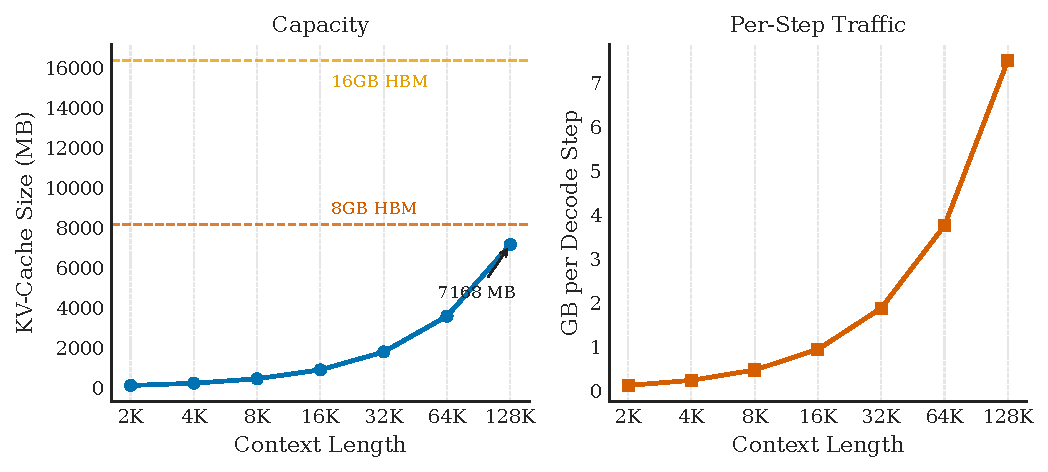
\includegraphics[width=\textwidth]{../paper_assets/figures/fig3_kv_cache_scaling.pdf}
\caption[上下文长度与 KV 缓存规模]{随着序列长度进入长上下文区间，KV 缓存处理规模迅速增长。}
\label{fig:scaling}
\end{figure}

图~\ref{fig:scaling} 展示了这一增长趋势。以 Qwen2.5-7B 级别模型为例，若采用 28 层、4 个 grouped-query KV 头、每头 128 维以及 FP16 存储，那么单个 $128{,}000$ token 请求的 KV 缓存大小将超过 7\,GB~\cite{vllm}。只有在系统愿意为单个请求分配大量加速器内存时，这个数字才是可接受的；而在多租户服务场景下，同样的线性增长会直接压缩并发度，并提高内存不足事件发生的概率。

CXL 可以提供所需容量，但流量需求依然严峻。如果系统以 20 tokens/s 的速度生成输出，并不断回取 GB 级历史状态，则所需互联带宽很快就会逼近甚至超过 PCIe/CXL 链路的实际能力~\cite{direct_cxl}。因此，长上下文服务同时面临内存容量和互联带宽两方面的压力。

\section{延迟剖析：时间究竟消耗在哪里}

为了分析 decode 时间的来源，可以将单个 token 的延迟拆分为三个部分：
\begin{enumerate}
    \item \textbf{矩阵计算：} 对模型权重和当前 token 状态执行的稠密算术。
    \item \textbf{反量化开销：} 在压缩整数表示与浮点计算格式之间进行转换的成本。
    \item \textbf{KV 缓存 I/O 遍历：} 访问与传输历史键和值的时间。
\end{enumerate}

\begin{figure}[htbp]
\centering
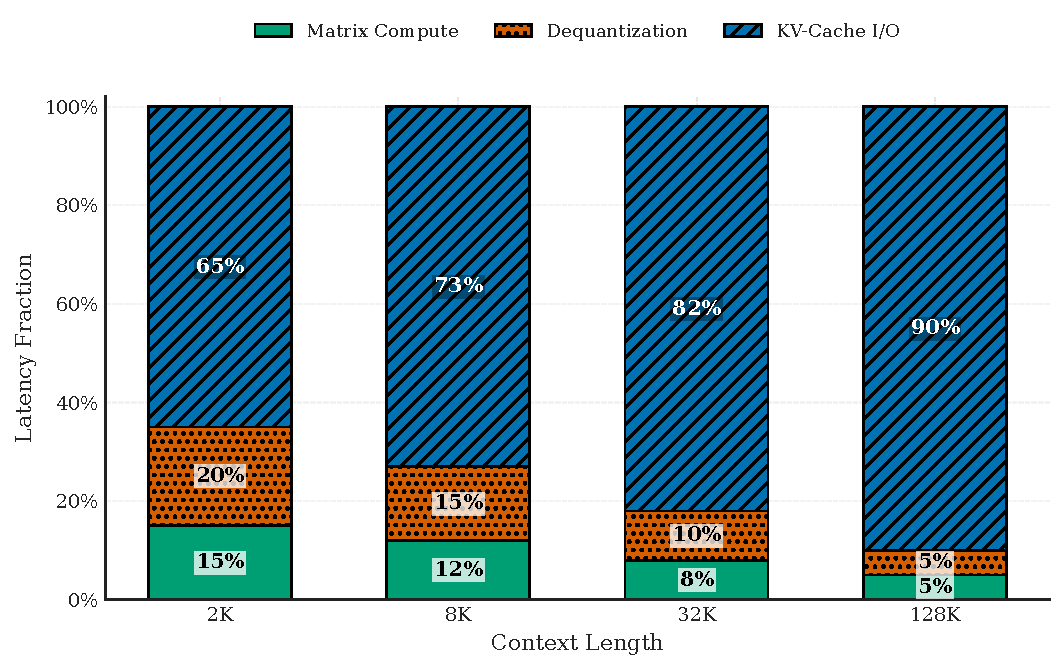
\includegraphics[width=\textwidth]{../paper_assets/figures/fig1_latency_breakdown.pdf}
\caption[不同上下文长度下的延迟构成]{不同上下文长度下的总体延迟构成。随着序列增长，KV 缓存遍历和格式转换逐渐成为主导项。}
\label{fig:latency}
\end{figure}

图~\ref{fig:latency} 表明，主导项会随上下文长度发生变化。在较短上下文下，矩阵计算仍然占据明显比例；但当上下文扩展到 32K 和 128K token 时，KV 缓存搬移已成为主要瓶颈，反量化也仍然是不可忽视的次级开销。这意味着，仅仅继续优化稠密计算单元，并不足以解决端到端 decode 的瓶颈。

\subsection{PIM 中格式失配的现实问题}

上述剖析说明，近内存注意力是一个很有前景的方向，因为它能够避免主机侧反复遍历 KV 缓存。但仍有第二个低效来源存在：量化存储与浮点非线性执行之间的失配。在很多实际部署中，为降低容量压力，KV 缓存张量会采用 INT8 等低精度格式存储~\cite{llm_outliers}。然而，现有许多近内存计算引擎仍假定采用浮点 Softmax 或其他代价较高的非线性数据通路~\cite{pim_quant}。如果没有整数域原生替代方案，系统仍需支付解包、转换、归一化和重新打包的代价。

\section{小结}

本章中的证据表明，一个面向长上下文的可扩展架构至少应满足两个要求。第一，KV 缓存注意力应尽可能在数据附近执行，以避免 decode 阶段持续压满主机互联。第二，注意力中的非线性部分应以能够保持量化数据通路的方式实现，从而避免反复进行浮点格式转换。本文后续章节将分别通过 LKC-CXL-PIM 和 DisaggKV 回应这两个要求。
